\begin{comment}
------------------------------------------------------------------------------------------
\end{comment}
\chapter{RO-SLAM}\label{ch:ro_slam}

Nachdem im vorherigen Kapitel die \Glspl{uwbm} für die Entfernungsmessung erstellt worden sind, wird jetzt nur noch eine Roboterplattform benötigt die mit einem Tag ausgestattet werden kann. Welche Hardwareplattform eingesetzt wird und von welchen Softwaremodulen diese gesteuert wird, folgt in den nächsten Abschnitten.

\begin{comment}
--------------------------------------------------------------------------------
- Einsatz mobiler Roboter in der Logistik am Beispiel des Robotino
	- http://www.r-moehrle.de/wissenschaftlicheArbeiten/robotino1.pdf
\end{comment}
\section{Roboterplattform}

Um die Messungen für den \Gls{roslam} aufzuzeichnen wird eine Roboterplattform benötigt auf der das \Gls{uwbm} montiert werden kann. Zusätzlich wird noch eine Reihe weiterer Sensoren benötigt, die im Folgenden vorgestellt werden.

Also Roboterplattform dient dabei der Robotino 2 von \textit{Festo Didactic}. Er gehört zur Klasse der holonomen Roboter, d.h. seinen Bewegungsmöglichkeiten unterliegen keinerlei Einschränkungen im zweidimensionalen Raum. Ermöglicht wird das, durch drei voneinander unabhängig arbeitenden omnidirektionalen Antriebseinheiten. Jede der drei Antriebseinheiten verfügt über einen Inkrementalgeber, mit dem sich abschätzen lässt, wie weit der Robotino gefahren ist. Um den Fehler der Inkrementalgeber in Kurvenfahrten zu reduzieren wird das digitale Gyroskop\footnote{Model: CruizCore XG1000 / XG1010} von \textit{Microinfinity} eingesetzt. Gesteuert wird der Robotino über eine \SI{300}{\MHz} starke Verarbeitungseinheit auf Basis eines Linux Betriebssystems mit einem Echtzeitkernel. \cite{festo2007robotinomanual}

An der höchsten Position des Robotinos befindet sich ein 2D--Laser--Entfernungsmesser\footnote{Model: TiM571-2050101} der Firma \textit{Sick}. Mit einem Öffnungswinkel von \SI{270}{\degree} und einem Arbeitsbereich von \SIrange{0.05}{25}{\meter} ist es möglich, genaue Belegungskarten der Umgebung zu erstellen. \cite{sick2016operatingmanual}

Die Verarbeitungseinheit des Robotinos ist leistungsfähig genug um die anstehenden Steuerungsaufgaben zu erfüllen. Jedoch ist diese von leistungshungrigen Anwendungen wie dem \Gls{roslam} überfordert. Aus diesem Grund wird eine zusätzliche Verarbeitungseinheit\footnote{Model: NUC5i7RYH} mit einem Intel Core i7\footnote{5. Generation des Intel Core i7-5557U Prozessor mit bis zu \SI{3.4}{\GHz}. \cite{intel2015nucproductbrief}} verwendet.

Die Fahrbefehle werden dem Robotino über einen Xbox Wireless Controller übermittelt.

\begin{figure}[h]
	\centering
	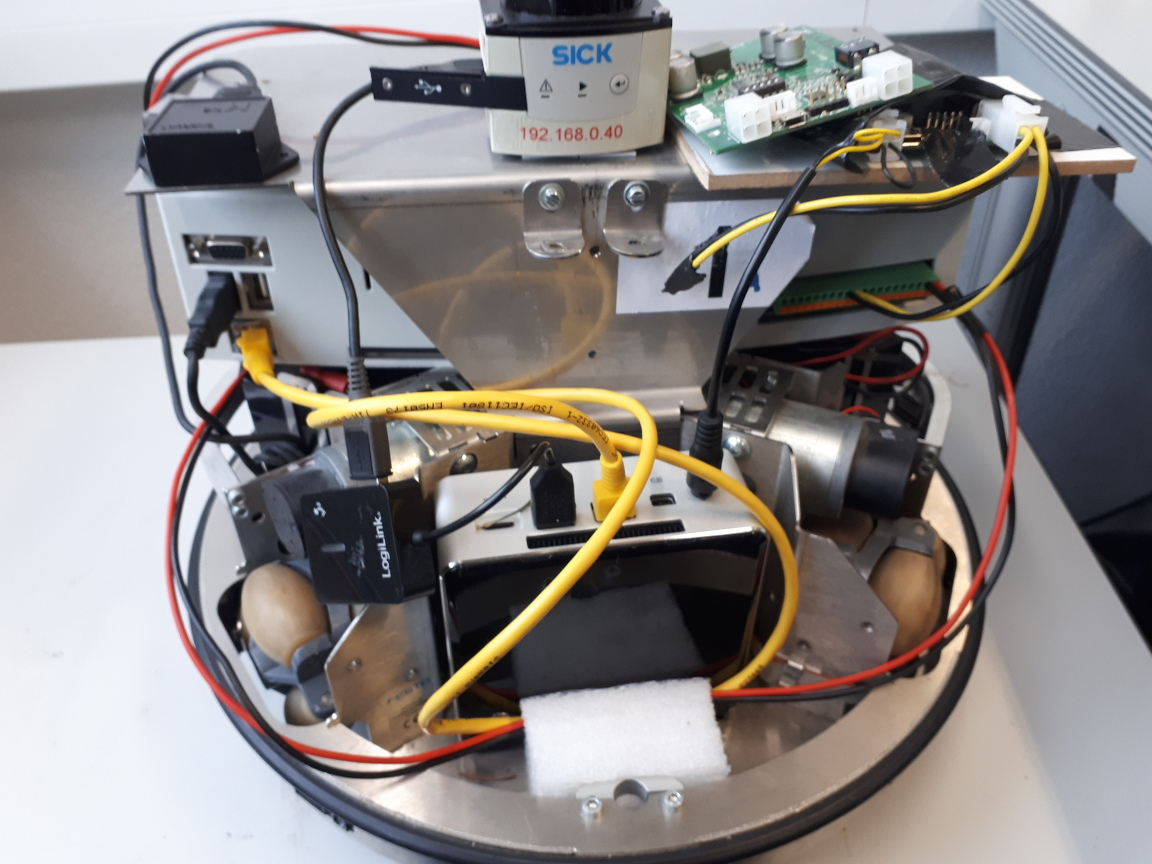
\includegraphics[width=0.5\textwidth]{robotino_front}
	\caption{[todo] Frontansicht des fertig aufgebauten Robotinos.}
	\label{fig:robotino_front}
\end{figure}


\begin{comment}
--------------------------------------------------------------------------------
- Kurzbeschreibung der Modulfunktion
- Welche Funktion erfüllt dieses Modul
- Welche ROS-Messages/-Topics/-Services bietet dieses Modul
\end{comment}
\section{Softwarearchitektur}

Die Softwarearchitektur ist unterteilt in drei Bereiche. Die absolut notwendigen Module für den \Gls{roslam} werden in den \Gls{ros}--Hauptmodulen besprochen. In den Abschnitt \Gls{ros}--Nebenmodulen werden die Module besprochen, die im Nachgang für die Auswertung der Ergebnisse benötigt werden. Und im letzten Abschnitt wird das \Gls{mrpt}--Framework vorgestellt, das den \Gls{roslam}--Algorithmus bereitstellt.


\begin{comment}
--------------------------------------------------------------------------------
- Begrifflichkeiten wie Topic, Sessage, Service usw. wurden bereits im Grundlagenkapitel geklärt.
- todo: Grundlagen ROS: URDF--Files, Lauch--Files, TF--Tree (odom, base_link, map?), Wofür braucht man Koordinatensystemtransformationen?
- todo: Übersicht über alle Module und deren Verbindung zu einander?
\end{comment}
\subsection{ROS--Hauptmodule}


\begin{comment}
--------------------------------------------------------------------------------
- \url{http://wiki.ros.org/robotino_node}
- todo: Service reset_odometry
\end{comment}
\subsubsection{Robotino--Steuerung}

Zur Steuerung der Roboterplattform muss die Verarbeitungseinheit Befehle zur Steuereinheit des Robotinos schicken. Diese Aufgabe erfüllt das \Gls{rosm} \textit{robotino\_node} aus dem Paket \textit{robotino\_node}. Über das Topic \textit{cmd\_vel} können die Geschwindigkeiten in X--/Y--Richtung und um die Z--Achse festgelegt werden. Um den Robotino zu stoppen, müssen alle drei Parameter auf den Wert Null gesetzt werden.

Um an die Informationen der Inkrementalgeber zu kommen muss das \Gls{rosm} \textit{robotino\_odometry\_node} aus dem Paket \textit{robotino\_node} gestartet werden. Nach dem Start steht das Topic \textit{odom} mit den aktuellen Werte der Inkrementalgeber zur Verfügung. Zusätzlich sorgt dieses Modul auch für die dynamische Transformation zwischen dem \textit{odom} und \textit{base\_link} Koordinatensystem.


\begin{comment}
--------------------------------------------------------------------------------
- \url{http://wiki.ros.org/robot_state_publisher}
- \url{http://wiki.ros.org/urdf}
\end{comment}
\subsubsection{Koordinatentransformation}

Neben den dynamischen Transformationen besteht der Robotino auch aus vielen statischen Transformationen. Hierzu gehört z.B. die Transformation vom Robotino--Mittelpunkt zum 2D--Laser--Entfernungsmesser oder \Gls{uwbm}. Diese statischen Transformationen werden in einer \Gls{urdf}--Datei einmalig gespeichert und dann über das \Gls{rosm} \textit{state\_publisher} aus dem Paket \textit{robot\_state\_publisher} zur Laufzeit bereitgestellt, siehe \autoref{fig:rviz_robotino_tf2}.

\begin{figure}[h]
	\centering
	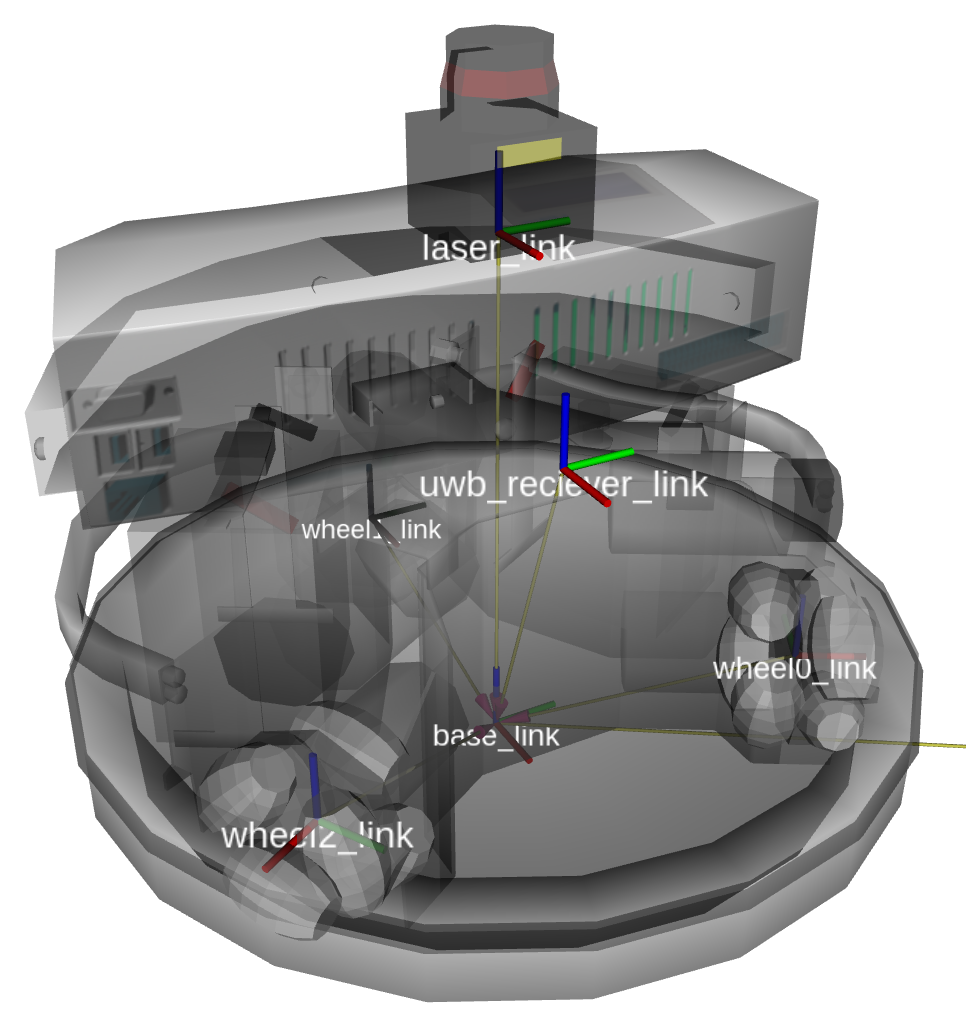
\includegraphics[width=0.5\linewidth]{rviz_robotino_tf2}
	\caption{Statische Transformationen des Robotino.}
	\label{fig:rviz_robotino_tf2}
\end{figure}


\begin{comment}
--------------------------------------------------------------------------------
- \url{http://wiki.ros.org/joy}
- todo: Referenz auf das lst:joy_node stehen lassen?
\end{comment}
\subsubsection{Teleoperation}

Um die Roboterplattform zu steuern wird ein Eingabegerät benötigt. Ein \textit{Xbox Wireless Controller} wird dabei als Eingabegerät verwendet. Zustandsänderungen am Eingabegerät werden über das \Gls{rosm} \textit{joy\_node} aus dem Paket \textit{joy} registriert und über das Topic \textit{joy} bereitgestellt. Das überwachte Eingabegerät wird über den Parameter \textit{dev} festgelegt, siehe \autoref{lst:joy_node}.

Mit den generischen Daten des Eingabegerätes kann die Roboterplattform jedoch nichts anfangen, diese benötigt eine Message vom Typ \textit{geometry\_msgs/Twist}. Die Transformation zwischen der Message \textit{sensor\_msgs/Joy} und \textit{geometry\_msgs/Twist} erfolgt durch das \Gls{rosm} \textit{xbox\_teleop.py} aus dem Paket \textit{ro\_slam\_with\_uwb}.


\begin{comment}
--------------------------------------------------------------------------------
\end{comment}
\subsubsection{UWB--Abstandsmessungen}

Die Abstandsmessungen zwischen dem \Gls{tag} und den vorhandenen \Glspl{anchor} werden durch das \Gls{uwbm} über die \Gls{usb}--Schnittstelle bereitgestellt. Die Daten werden dann von dem \Gls{rosm} \textit{beacon\_publisher.py} aus dem Paket \textit{ro\_slam\_with\_uwb} aufgefangen und auf den Topics \textit{beacon} und \textit{beacon\_raw} veröffentlicht. Das erste Topic ist vom Typ \textit{mrpt\_msgs/ObservationRangeBeacon} und wird von dem \Gls{mrpt}--Modul für den \Gls{roslam} benötigt. Das zweite Topic wird die Auswertung der Abstandmessungen im \autoref{ch:eval} benötigt und ist vom Typ \textit{ro\_slam\_with\_uwb/Beacon}.


\begin{comment}
--------------------------------------------------------------------------------
\end{comment}
\subsection{ROS--Hilfsmodule}


\begin{comment}
--------------------------------------------------------------------------------
- \url{http://wiki.ros.org/sick_tim}
\end{comment}
\subsubsection{2D--Laser--Entfernungsmesser}

Der 2D--Laser--Entfernungsmesser gehört zu einem der am häufigsten verwendeten Sensoren für die präzise visuelle Erfassen der Umwelt. Für mehrere der nachfolgenden \Gls{rosm} ist eine 2D--Laser--Entfernungsmessung eine zwingende Voraussetzung. Um die Daten dem \Gls{ros}--System bereitzustellen wird das \Gls{rosm} \textit{sick\_tim551\_2050001} aus dem Paket \textit{sick\_tim} verwendet. Dieses Modul stellt über dem Topic \textit{scan} mit einer Rate von \SI{15}{\hertz} Messages vom Typ \textit{sensor\_msgs/LaserScan} bereit.


\begin{comment}
--------------------------------------------------------------------------------
- \url{http://wiki.ros.org/hector_mapping}
\end{comment}
\subsubsection{Belegungskarten}

Das erste \Gls{rosm}, das von der 2D--Laser--Entfernungsmessung Gebrauch macht, ist das \textit{hector\_mapping} aus dem Paket \textit{hector\_mapping}. Mit diesem Modul können präzise Belegungskarten (engl. Occupancy Grid Map) erstellt werden, die für jede Koordinate der Karte festlegen ob diese durch ein Hindernis belegt (schwarz) oder frei (weiß) ist. Bereiche die von Hindernissen verdeckt sind oder außerhalb der Sensorreichweite liegen, werden als unbestimmt (grau) markiert, siehe \autoref{fig:rviz_occupancy_grid_map}. In \Gls{ros} werden Belegungskarten mit dem Message Typ \textit{nav\_msgs/OccupancyGrid} repräsentiert.

Zu den wichtigsten Parametern zählt die minimale und maximale Sensorreichweite (\textit{laser\_min\_dist} bzw. \textit{laser\_max\_dist}) die für die Kartenerstellung berücksichtigt wird und die Auflösung (\textit{map\_resolution}) einer Zelle in der Karte.

\begin{figure}[h]
	\centering
	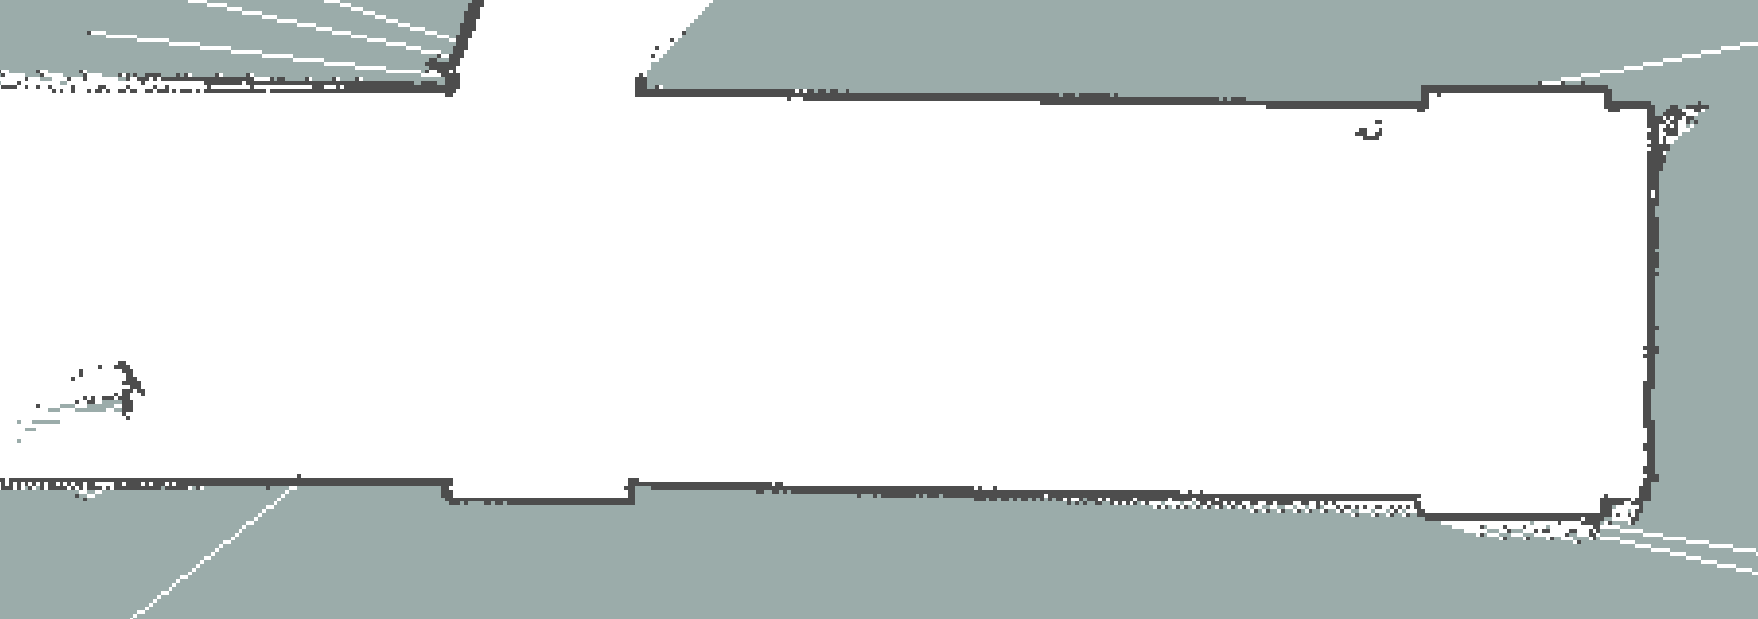
\includegraphics[width=0.9\linewidth]{rviz_occupancy_grid_map}
	\caption{Die Belegungskarte der Messstrecke.}
	\label{fig:rviz_occupancy_grid_map}
\end{figure}
 

\begin{comment}
--------------------------------------------------------------------------------
- \url{http://wiki.ros.org/hector_trajectory_server}
- \url{http://docs.ros.org/api/nav_msgs/html/msg/Path.html}
\end{comment}
\subsubsection{Trajektorie}

Neben den Entfernungsinformationen wertet der \Gls{roslam} auch die Daten der Odometrie aus. Als Quelle für die Odometrie dienen dabei die Inkrementalgeber des Robotino. Im nächsten Abschnitt werden weitere Quellen für die Odometrie vorgestellt. Um nun die Güte der Odometrie--Quellen zu vergleichen, wird die verfahrene Trajektorie jeder Quelle benötigt. Diese Informationen werden von dem \Gls{rosm} \textit{hector\_trajectory\_server} aus dem Paket {hector\_trajectory\_server} bereitgestellt. Die Daten liegen dabei als Message vom Typ \textit{nav\_msgs/Path} bereit und können in die Belegungskarte integriert werden, siehe \autoref{fig:rviz_trajektorie}.

\begin{figure}[h]
	\centering
	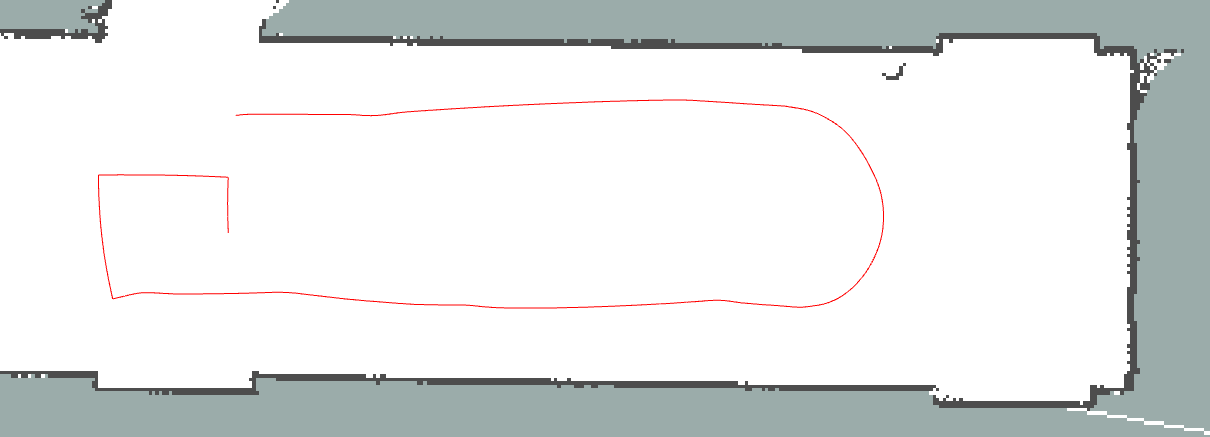
\includegraphics[width=0.9\linewidth]{rviz_trajektorie}
	\caption{Die Trajektorie einer Messfahrt des Robotino.}
	\label{fig:rviz_trajektorie}
\end{figure}


\begin{comment}
--------------------------------------------------------------------------------
- \url{http://wiki.ros.org/rf2o}
- \url{http://wiki.ros.org/laser_scan_matcher}

rf2o\_laser\_odometry
Estimation of 2D odometry based on planar laser scans. Useful for mobile robots with innacurate base odometry. For full description of the algorithm, please refer to: Planar Odometry from a Radial Laser Scanner. A Range Flow-based Approach. ICRA 2016 Available at: http://mapir.isa.uma.es/mapirwebsite/index.php/mapir-downloads/papers/217


laser\_scan\_matcher
An incremental laser scan matcher, using Andrea Censi's Canonical Scan Matcher (CSM) implementation. See the web site for more about CSM. NOTE the CSM library is licensed under the GNU Lesser General Public License v3, whereas the rest of the code is released under the BSD license.

The laser_scan_matcher package is an incremental laser scan registration tool. The package allows to scan match between consecutive sensor_msgs/LaserScan messages, and publish the estimated position of the laser as a geometry_msgs/Pose2D or a tf transform.

The package can be used without any odometry estimation provided by other sensors. Thus, it can serve as a stand-alone odometry estimator. Alternatively, you can provide several types of odometry input to improve the registration speed and accuracy.

    <node
        if="$(arg enable_laser_scan_matcher)"
        pkg="laser_scan_matcher" type="laser_scan_matcher_node" name="laser_scan_matcher_node"
        output="screen">

        <param name="base_frame" value="base_link"/>
        <param name="fixed_frame" value="odom" />
        <param name="use_odom" value="true" />
        <param name="use_imu" value="false" />
    </node>

- Vergleichen der Roboter--Odometrie mit zwei Laser--Odometrien.

\end{comment}
\subsubsection{Laser--Odometrie}

Wie bereits im vorherigen Abschnitt erwähnt, werden hier zwei weitere Quelle für die Odometrie vorgestellt. Beide \Glspl{rosm} nutzen nur die Daten der 2D--Laser--Ent\-fern\-ungs\-mes\-sung um eine Schätzung für die aktuelle Pose zu erstellen. Bei dem ersten handelt es sich um den \textit{laser\_scan\_matcher\_node} aus dem Paket \textit{laser\_scan\_matcher} und bei dem zweiten um den \textit{rf2o\_laser\_odometry\_node} aus dem Paket \textit{rf2o\_laser\_odometry}.


\begin{comment}
--------------------------------------------------------------------------------
\subsubsection{Vergleich der Trajektorie von Odom und rf2o}

- Trajektorie der Robotino--Odometry bestimmen.
- Herausfiltern der Odometry Nachrichten aus den Bag--Dateien
- Odometry aus den Laser--Scans bestimmen und Trajektorie aufzeichen.
- Trajektorien vergleichen
\end{comment}




\begin{comment}
--------------------------------------------------------------------------------
\subsubsection{gmapping}

- This package contains a ROS wrapper for OpenSlam's Gmapping.
- The gmapping package provides laser-based SLAM (Simultaneous Localization and Mapping), as a ROS node called slam\_gmapping.
- Using slam\_gmapping, you can create a 2-D occupancy grid map from laser and pose data collected by a mobile robot.
\url{http://wiki.ros.org/gmapping}

Benötigt eine TF--Transformation zwischen base\_link und odom. Mittels der Odometry und dem Laser--Scans erzeugt er eine TF--Transformation zwischen map und odom.
\end{comment}







\begin{comment}
--------------------------------------------------------------------------------
- ros
	- <node pkg="mrpt_rbpf_slam" type="mrpt_rbpf_slam" name="mrpt_rbpf_slam" output="screen" />
- mrpt
	- rbpf_slam.ini
- https://www.mrpt.org/list-of-mrpt-apps/application-rbpf-slam/
	- It is actually a front-end to the class mrpt::slam::CMetricMapBuilderRBPF. All the parameters to the algorithm are passed through a configuration file in the command line. The filter processes actions and observations from a rawlog file and optionally generates a number of files describing the evolution of the filter and the maps.
	- The mathematical background of RBPF-based SLAM and to see an updated list of the implemented RBPF-SLAM solutions can be found in this tutorial page.
	- http://mrpt.ual.es/reference/devel/classmrpt_1_1slam_1_1_c_metric_map_builder_r_b_p_f.html
	- MC / SOG
	- https://www.mrpt.org/tutorials/slam-algorithms/rangeonly_slam/
	
	
pub_map_ = n_.advertise<nav_msgs::OccupancyGrid>("map", 1, true);
// robot pose
pub_Particles_ = n_.advertise<geometry_msgs::PoseArray>("particlecloud", 1, true);
 / ro particles poses
pub_Particles_Beacons_ = n_.advertise<geometry_msgs::PoseArray>("particlecloud_beacons", 1, true);
	
if (lstSources[i].find("scan") != std::string::npos)
    {
      sensorSub_[i] = n_.subscribe(lstSources[i], 1, &PFslamWrapper::laserCallback, this);
    }
    else
    {
      sensorSub_[i] = n_.subscribe(lstSources[i], 1, &PFslamWrapper::callbackBeacon, this);
    }
    
    
void PFslamWrapper::odometryForCallback(CObservationOdometry::Ptr& _odometry, const std_msgs::Header& _msg_header)
{
  mrpt::poses::CPose3D poseOdom;
  if (this->waitForTransform(poseOdom, odom_frame_id, base_frame_id, _msg_header.stamp, ros::Duration(1)))
	
\end{comment}
\subsection{MRPT Modul [todo]}








